
\section{Consuntivo Finale}
\label{consFinale}
\subsection{Consuntivo Ruoli}
La seguente sezione illustra la situazione riguardante le risorse e il budget finanziario che il gruppo \authorName{} ha utilizzato per la realizzazione del progetto \project{}.
\\
La seguente tabella riporta le ore effettivamente impiegate con i relativi costi; tra parentesi vengono indicate le differenze rispetto al preventivo (con segno positivo si indicano quanto in più è stato utilizzato rispetto alla pianificazione, con segno negativo invece quanto in meno è stato utilizzato rispetto a quanto pianificato). La prima tabella riporta le differenze totali, comprensive anche della Fase A (FA) mentre la seconda tabella riporta le differenze remunerabili ovvero quelle imputabili al proponente per la realizzazione del progetto.
\begin{table}[!h]
		\centering
		\begin{tabular}{|l|c|c|}
			\hline
			Ruolo & Ore & Costo\\
			\hline
			Amministratore & 42 (-11) & 840 (-220)\\
			Responsabile & 41 (-9) & 1.230 (-270)\\
			Analista & 106 (-8) & 2.650 (-200)\\
			Verificatore & 279 (-2) & 6.138 (-44)\\
			Progettista & 239 (+15) & 3.585 (+225)\\
			Programmatore & 165 (+33) & 2.475 (+495)\\	
			\hline
			consuntivo & 872 & 16.918\\
			preventivo & 854 & 16.932\\
			differenza & +18 & -14\\
			\hline			
		\end{tabular}
		\caption{Consuntivo per Ruolo, totale}
		\label{consuntivoFinTot}
	\end{table}
\\ Viene riportato di seguito, il monte ore per ruolo preventivato e quello effettivamente utilizzato ovvero consuntivato comprensivo anche della fase A (FA).

\begin{figure}[!h]
	\centering
	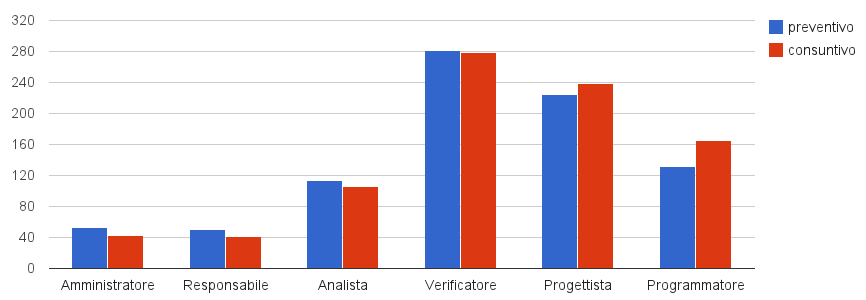
\includegraphics[width=1.1\textwidth] {./content/Immagini/totaliTot}
	\caption{Bilancio per ruolo, totali}
	\label{biltot}
\end{figure}	 
	
\begin{table}[!h]
		\centering
		\begin{tabular}{|l|c|c|}
			\hline
			Ruolo & Ore & Costo\\
			\hline
			Amministratore & 23 (-10) & 460 (-200)\\
			Responsabile & 22 (-10) & 660 (-300)\\
			Analista & 42 (-7) & 1.050 (-175)\\
			Verificatore & 237 (-3) & 5.214 (-66)\\
			Progettista & 239 (+15) & 3.585 (+225)\\
			Programmatore & 165 (+33) & 2.475 (+495)\\	
			\hline
			consuntivo & 728 & 13.444\\
			preventivo & 710 & 13.465\\
			differenza & +18 & -21\\
			\hline			
		\end{tabular}
		\caption{Consuntivo per Ruolo, remunerabile}
		\label{consuntivoFinRem}
	\end{table}
	
\pagebreak Viene riportato di seguito, il monte ore per ruolo preventivato e quello effettivamente utilizzato ovvero consuntivato imputabile al proponente, non comprensivo della fase A (FA).

\begin{figure}[!h]
	\centering
	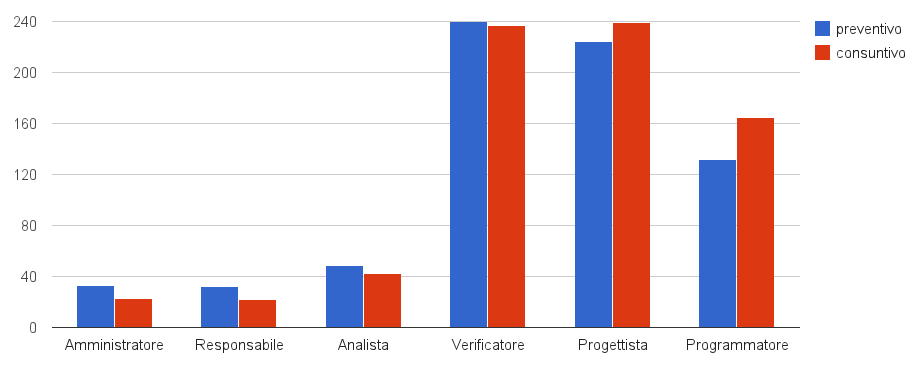
\includegraphics[width=1.1\textwidth] {./content/Immagini/totaliRemun}
	\caption{Bilancio per ruolo, remunerabile}
	\label{bilRem}
\end{figure}	
\pagebreak

\subsection{Consuntivo Risorse}
\label{consRisorse}
La seguente sezione presenta il consuntivo riguardante le risorse impiegate per ricoprire i ruoli individuati al fine di realizzare il progetto commisionato.
Le tabelle seguenti mostrano le ore realmente impiegate da ogni risorsa nei diversi ruoli riportando tra parentesi la differenza tra le ore preventivate e quelle effettivamente ricoperte.
La prima tabella illustra la situazione complessiva, considerando anche le ore utilizzate nella fase A (FA), mentre la seconda mostra la situazione oraria remunerabile, ovvero a carico del proponente, escludendo dunque la fase A (FA).

\begin{table} [!h]
\tableResource
Adami Alberto & 10 (0) &5 (0) & 15 (-2) & 51 (+2) &35 (+3) &8 (+1) & 124 (+4)\\
Bissacco Nicolò & 9 (-1)& 4 (0)& 14 (0)& 45 (-7)& 33 (+2)& 19 (+9)& 124 (+3)\\
Feltre Beatrice & 4 (-7)& 9 (+1)& 10 (-2)&48 (+8)&48 (+4)&4 (-3)& 123 (+1)\\
Luisetto Luca & 4 (0)& 4 (-6)& 14 (+1) & 38 (-1) &31 (0) & 35 (+9)& 126 (+3)\\
Magnabosco Nicola &6 (-3)& 10 (0)&15 (-3) & 22 (-2)&26 (+3) & 47 (+7) & 126 (+2)\\
Martignago Jimmy & 2 (0)& 2 (0)& 24 (-2)& 36 (-5) &43 (+6) & 18 (+4)& 125 (+3)\\
Scapin Davide & 7 (0)&7 (-4) & 14 (0) & 39 (+3) &23 (-3) &34 (+6) & 124 (+2)\\ \hline
\end{tabular}\caption{Ore a Componente per Ruolo finali, totali} \end{center}
\end{table}
il grafico seguente riporta in modo sintetico  i dati illustrati dalla precedente tabella.
\begin{figure}[!h]
	\centering
	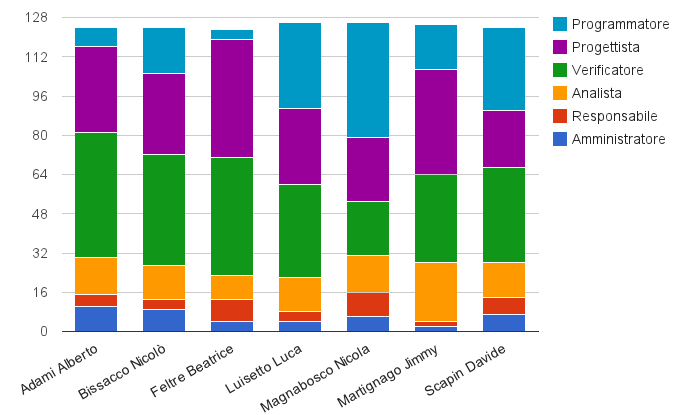
\includegraphics[width=1.1\textwidth] {./content/Immagini/ruoliTotali}
	\caption{Risorse per Ruolo, totali}
	\label{risTot}
\end{figure}	
\pagebreak
\begin{table} [!h]
\tableResource
Adami Alberto &  &5 (0) &  8(-2)& 48 (+2) &35 (+3) &8 (+1) & 104 (+4)\\
Bissacco Nicolò & & & 7 (0)& 45 (-7)& 33 (+2)& 19 (+9)& 104 (+4)\\
Feltre Beatrice & 4 (-7)& & &48 (+8) &48 (+4) &4 (-3)& 104 (+2)\\
Luisetto Luca & 4 (0)& 4 (-6) & & 30 (-1) &31 (0) & 35 (+9)& 104 (+2)\\
Magnabosco Nicola &6 (-3)& 4 (0)&15 (-3)  & 6 (-3)& 26 (+3) & 47 (+7) & 104 (+1)\\
Martignago Jimmy & 2 (0)&  2 (0)& 9 (-2)& 30 (-5)&43 (+6)& 18 (+4)& 104 (+3)\\
Scapin Davide & 7 (0)&7 (-4)& 3 (0)& 30 (+3)&23 (-3) &34 (+6) & 104 (+2)\\ \hline
\end{tabular}\caption{Ore a Componente per Ruolo finali, remunerabili} \end{center}
\end{table}

il grafico seguente riporta in modo sintetico  i dati illustrati dalla precedente tabella.
\begin{figure}[!h]
	\centering
	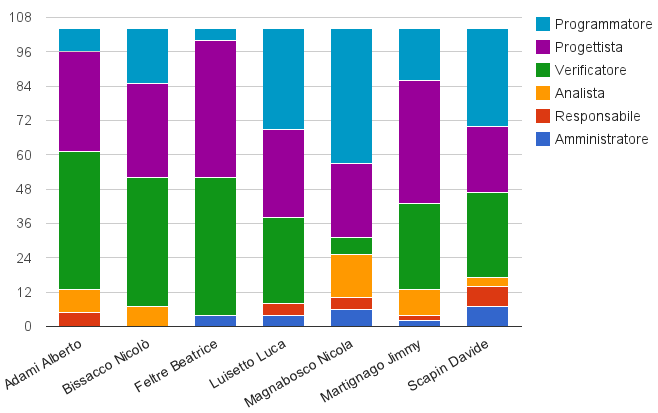
\includegraphics[width=1.1\textwidth] {./content/Immagini/ruoliRem.png}
	\caption{Risorse per Ruolo, remunerabili}
	\label{risTot}
\end{figure}	
\pagebreak
\subsection{Consuntivo economico e conclusioni}
\label{consFin}
I grafici di seguito, illustrano i dati monetari riportati rispettivamente nella tabella \ref{consuntivoFinTot} per i costi totali comprensivi della fase A (FA) e nella tabella \ref{consuntivoFinRem} per i costi imputabili al proponente ovvero esclusi i costi sostenuti nella fase A (FA), suddivisi per ruoli.
\begin{figure}[!h]
	\centering
	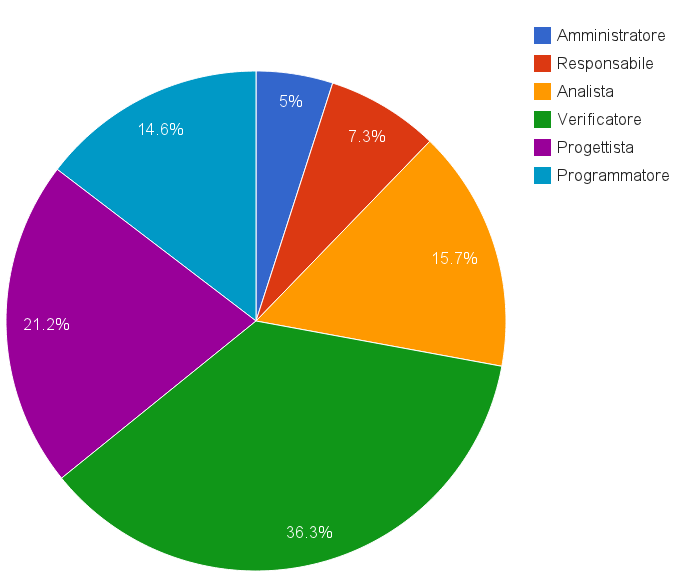
\includegraphics[width=0.8\textwidth] {./content/Immagini/costiTotFin.png}
	\caption{Costi totali suddivisi per ruoli}
	\label{costiTot}
\end{figure}	

\begin{figure}[!h]
	\centering
	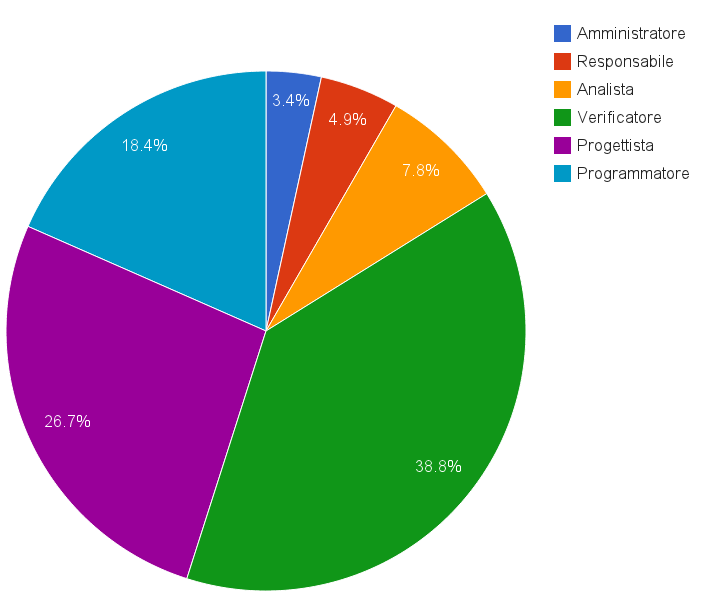
\includegraphics[width=0.8\textwidth] {./content/Immagini/costiRem.png}
	\caption{Costi remunerabili suddivisi per ruoli}
	\label{costiRem}
\end{figure}	
\subsubsection{Conclusioni}
Come si evince dalle tabelle precedenti, le ore totali per la realizzazione del progetto si sono leggermente discostate da quanto pianificato all'avvio del progetto. Questo è dovuto innanzittutto all'inesperienza da parte dei componenti del gruppo nel coinvolgimento di un'attività di certe dimensioni che ha portato a sovrastimare o sottostimare la presenza di alcuni ruoli. Altre cause invece legate al flusso degli eventi che hanno rallentato i lavori.
Si sono riuscite a garantire almeno il 30\% (più precisamente circa il 38\%) delle ore totali al ruolo del verificatore volte a migliorare la qualità dei processi e dei prodotti in ingresso alle varie revisioni. 
\\ Nonostante tutto, si è riusciti a non eccedere il budget pianificato (\EUR{13.465}) con un impegno produttivo da parte di ogni componente di \textbf{104 ore} per un costo complessivo di \textbf{\EUR{13.444}}.